% Created with jtex v.1.0.8
\documentclass{article}
\usepackage{arxiv}

\usepackage[utf8]{inputenc} % allow utf-8 input
\usepackage[T1]{fontenc}    % use 8-bit T1 fonts
\usepackage{hyperref}       % hyperlinks
\usepackage{url}            % simple URL typesetting
\usepackage{datetime}       % show dates in the title block
\usepackage{booktabs}       % professional-quality tables
\usepackage{amsfonts}       % blackboard math symbols
\usepackage{nicefrac}       % compact symbols for 1/2, etc.
\usepackage{microtype}      % microtypography
\usepackage{graphicx}
\usepackage{natbib}
\usepackage{doi}
\usepackage{xcolor}

%%%%%%%%%%%%%%%%%%%%%%%%%%%%%%%%%%%%%%%%%%%%%%%%%%
%%%%%%%%%%%%%%%%%%%%  imports  %%%%%%%%%%%%%%%%%%%
\usepackage{amsmath}
%%%%%%%%%%%%%%%%%%%%%%%%%%%%%%%%%%%%%%%%%%%%%%%%%%
\usepackage{glossaries}
\makeglossaries

%%%%%%%%%%%%%%%%%%%%%%%%%%%%%%%%%%%%%%%%%%%%%%%%%%
%%%%%%%%%%%%%%%%%%%  acronyms  %%%%%%%%%%%%%%%%%%%
\newacronym{fchnn}{fcHNN}{functional connectome-based Hopfield Neural Network}
\newacronym{hnn}{HNN}{Hopfield Neural Network}
\newacronym{ann}{ANN}{Artificial Neural Network}
\newacronym{fmri}{fMRI}{functional Magnetic Resonance Imaging}
\newacronym{abide}{ABIDE}{Autism Brain Imaging Data Exchange}
\newacronym{asd}{ASD}{Autism Spectrum Disorder}
\newacronym{dl}{dl}{dorsolateral}
\newacronym{pfc}{PFC}{Prefrontal Cortex}
\newacronym{mcc}{MCC}{Middle Cingulate Cortex}
\newacronym{acc}{ACC}{Anterior Cingulate Cortex}
\newacronym{pg}{pg}{perigenual}
\newacronym{dm}{dm}{dorsomedial}
\newacronym{stg}{STG}{Superior Temporal Gyrus}
\newacronym{itg}{ITG}{Inferior Temporal Gyrus}
\newacronym{caud/acc}{Caud/Acc}{Caudate-Accumbens}
\newacronym{sm}{SM}{Sensorimotor}
\newacronym{v1}{V1}{Primary Visual}
\newacronym{a1}{A1}{Primary Auditory}
%%%%%%%%%%%%%%%%%%%%%%%%%%%%%%%%%%%%%%%%%%%%%%%%%%

\hypersetup{colorlinks = true,
linkcolor = purple,
urlcolor  = blue,
citecolor = cyan,
anchorcolor = black}

\title{Attractor states of the functional brain connectome orchestrate large-scale brain dynamics}

\newdate{articleDate}{1}{11}{2023}
\date{\displaydate{articleDate}}

\makeatletter
\let\@fnsymbol\@arabic
\makeatother

\author{Robert Englert\\
Department of Diagnostic and Interventional Radiology and Neuroradiology,  University Medicine Essen, Germany\\\AND
Balint Kincses\\
Department of Neurology, University Medicine Essen, Germany\\\AND
Raviteja Kotikalapudi\\
Department of Neurology, University Medicine Essen, Germany\\\AND
Giuseppe Gallitto\\
Department of Neurology, University Medicine Essen, Germany\\\AND
Jialin Li\\
Department of Neurology, University Medicine Essen, Germany\\Max Planck School of Cognition, Leipzig, Germany\\\AND
Kevin Hoffschlag\\
Department of Neurology, University Medicine Essen, Germany\\\AND
Choong-Wan Woo\\
Center for Neuroscience Imaging Research, Institute for Basic Science, Suwon, South Korea\\Department of Biomedical Engineering, Sungkyunkwan University, Suwon, South Korea\\\AND
Tor D. Wager\\
Department of Psychological and Brain Sciences, Dartmouth College, Hanover, NH, USA\\\AND
Dagmar Timmann\\
Department of Neurology, University Medicine Essen, Germany\\Center for Translational Neuro- and Behavioral Sciences (C-TNBS), University Medicine Essen, Germany\\\AND
Ulrike Bingel\\
Department of Neurology, University Medicine Essen, Germany\\Center for Translational Neuro- and Behavioral Sciences (C-TNBS), University Medicine Essen, Germany\\\AND
\href{https://orcid.org/0000-0002-2942-0821}{
\includegraphics[scale=0.06]{orcid.pdf}}\hspace{1mm}Tamas Spisak\footnotemark[1]\\
Department of Diagnostic and Interventional Radiology and Neuroradiology,  University Medicine Essen, Germany\\Center for Translational Neuro- and Behavioral Sciences (C-TNBS), University Medicine Essen, Germany\\}

% Uncomment to override  the `A preprint' in the header
\renewcommand{\headeright}{manuscript draft}
\renewcommand{\undertitle}{}
\renewcommand{\shorttitle}{Manuscript}

%% Add PDF metadata to help others organize their library
%% Once the PDF is generated, you can check the metadata with
%% $ pdfinfo template.pdf
\hypersetup{
pdftitle={\@title},
pdfsubject={},
pdfauthor={\@author},
pdfkeywords={},
addtopdfcreator={Written in Curvenote}
}

\begin{document}
\maketitle
\footnotetext[1]{Correspondence to: tamas.spisak@uk-essen.de}

\begin{abstract}
Understanding large-scale brain dynamics is a grand challenge in neuroscience.
We propose functional connectome-based Hopfield neural networks (fcHNNs) as a model of macro-scale brain dynamics, arising from recurrent activity flow among brain regions. An fcHNN is neither optimized to mimic certain brain characteristics, nor trained to solve specific tasks; its weights are simply initialized with empirical functional connectivity values.
In the fcHNN framework, brain dynamics are understood in relation to so-called attractor states, i.e. neurobiologically meaningful low-energy activity configurations.
Analyses of 7 distinct datasets demonstrate that fcHNNs can accurately reconstruct and predict brain dynamics under a wide range of conditions, including resting and task states and brain disorders.
By establishing a mechanistic link between connectivity and activity, fcHNNs offers a simple and interpretable  computational alternative to conventional descriptive analyses of brain function. Being a generative framework, fcHNNs can yield mechanistic insights and hold potential to uncover novel treatment targets.
\end{abstract}

\keywords{}

\textbf{Key Points:}

\begin{itemize}
\item We present a simple yet powerful computational model for large-scale brain dynamics
\item The model uses a functional connectome-based Hopfield artificial neural network (\acrshort{fchnn}) architecture to compute recurrent "activity flow" through the functional brain connectome
\item Fc\acrshort{hnn}s accurately reconstruct the dynamic repertoire of the brain in resting conditions
\item Fc\acrshort{hnn}s conceptualize both task-induced and pathological changes in brain activity as a non-linear shift in these dynamics
\item Our approach is validated using data from seven studies involving approximately 1000 participants
\end{itemize}

\subsection{Introduction}

Brain function is characterized by the continuous activation and deactivation of anatomically distributed neuronal
populations \citep{buzsaki2006rhythms}.
Irrespective of the presence or absence of explicit stimuli, brain regions appear to work in concert, giving rise to a
rich and spatiotemporally complex fluctuation \citep{bassett2017network}.
This fluctuation is neither random, nor stationary over time \citep{liu2013time, zalesky2014time}.
It is organized around largee-scale gradints \citep{margulies2016situating, huntenburg2018large} and exhibits quasi-periodic properties, with a limited number of recurring patterns known as "brain states" \citep{greene2023everyone, vidaurre2017brain, liu2013time}.

A wide variety of descriptive techniques have been previously employed to characterize whole-brain dynamics \citep{smith2012temporally, vidaurre2017brain, liu2013time, chen2018human}.
These efforts have provided accumulating evidence not only for the existence of dynamic brain states but also for their clinical
significance \citep{hutchison2013dynamic, barttfeld2015signature, meer2020movie}.
However, the underlying driving forces remain elusive due to the descriptive nature of such studies.

Conventional computational approaches attempt to solve this puzzle by going all the way down to the biophysical properties of single neurons, and aim to construct a model of larger neural populations, or even the entire brain
\citep{breakspear2017dynamic}.
These approaches have shown numerous successful applications \citep{murray2018biophysical, kriegeskorte2018cognitive, heinz2019towards}.
However, the estimation of the vast number of free parameters in such models hambers their ability to effectively bridge the gap between explanations at the level of single neurons and the complexity of behavior \citep{breakspear2017dynamic}.
Recent efforts using coarse-grained brain network models \citep{schirner2022dynamic, schiff1994controlling, papadopoulos2017development} and linear network control theory  \citep{chiem2021structure, scheid2021time, gu2015controllability} opted to trade biophysical fidelity to phenomenological validity. The challenge for such models lies in modelling the relation between the structural wiring of the brain and functional connectivity.
The "neuroconnectionist" approach, on the other hand, \citep{doerig2023neuroconnectionist} aims at "cognitive/behavioral fidelity" \citep{kriegeskorte2018cognitive}, by using artificial neural networks (\acrshort{ann}s) that are trained to perform various tasks, as brain models. However, the need to train \acrshort{ann}s for specific tasks inherently limits their ability to explain task-independent, spontaneous neural dynamics \citep{richards2019deep}.

Here we propose a novel approach that combines the advantages of large-scale network models and neuroconnectionism, to investigate brain dynamics.
Similar to neuroconnectionism, we utilize an \acrshort{ann} as a high-level computational model of the brain.
However, our model is not explicitly trained for a specific task. Instead, we set its weights empirically, with data based on the "activity flow" \citep{cole2016activity, ito2017cognitive} across regions within the functional brain connectome, as measured with functional magnetic resonance imaging (\acrshort{fmri}, Figure~\ref{concept}B).

Specifically, we employ a continuous-space Hopfield neural network (\acrshort{hnn}) \citep{hopfield1982neural, krotov2023new}, with its nodes representing large-scale brain areas, and its weights initialized with the functional connectivity values between these areas.
Based on the topology of the functional connectome, this architecture establishes an energy level for any arbitrary activation patterns and determines a "trajectory of least action" towards one of the finite number of stable patterns, known as \textit{attractor states}, that minimize this energy.
In this simplistic yet powerful framework, brain dynamics can be conceptualized as an intricate, high-dimensional path on the energy landscape (Figure~\ref{concept}C), arising from the activity flow \citep{cole2016activity} within the functional connectome and constrained by the "gravitational pull" of the attractor states of the system.
Given its generative nature, the proposed model offers testable predictions for the effect of various perturbations and alterations of these dynamics, from task-induced activity, to changes related to brain disorders.

\begin{figure}[!htbp]
\centering
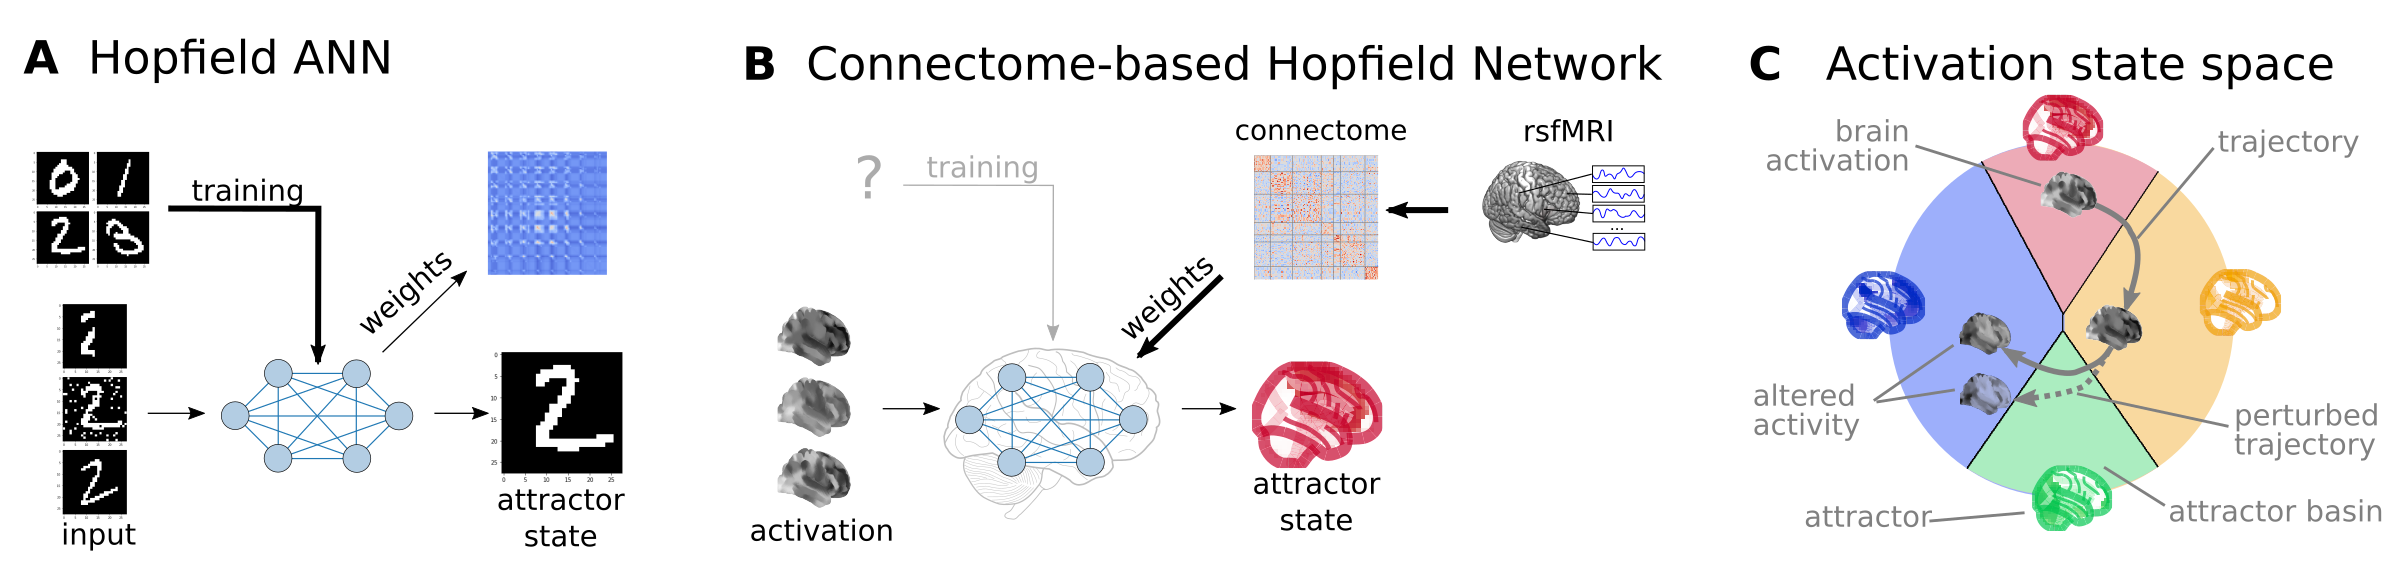
\includegraphics[width=0.7\linewidth]{files/concept-0b76fbed89f4b539cbde8c994d21e370.png}
\caption[]{\textbf{Connectome-based Hopfield networks as models of macro-scale brain dynamics.} \newline
\newline

\textbf{A} Hopfield artificial neural networks (\acrshort{hnn}s)  are a form of recurrent artificial neural networks that serve as content-addressable ("associative") memory systems. Hopfield networks can be trained to store a finite number of patterns (e.g. via Hebbian learning a.k.a. "fire together -  wire together"). During the training procedure, the weights of the \acrshort{hnn} are trained so that the stored
patterns become stable attractor states of the network. Thus, when the trained network is presented partial, noisy or corrupted variations of the stored patterns, it can effectively reconstruct the original pattern via an iterative relaxation procedure that converges to the attractor states.
\textbf{B} We consider regions of the brain as nodes of a Hopfield network. Instead of training the Hopfield network to
specific tasks, we set its weights empirically, with the interregional activity flow estimated via functional
brain connectivity. Capitalizing on strong analogies between the relaxation rule of Hopfield networks and the
activity flow principle that links activity to connectivity in brain networks, we propose the resulting
functional connectome-based Hopfield neural network (\acrshort{fchnn}) as a computational model for macro-scale brain dynamics.\newline
\textbf{C} The proposed computational framework assigns an energy level, an attractor state and a position in a
low-dimensional embedding to brain activation patterns. Additionally, it models how the entire state-space of viable activation patterns is restricted by the dynamics of the system and how alterations in activity and/or connectivity modify these dynamics.}
\label{concept}
\end{figure}

In the present work, we use \acrshort{hnn}s to explore the functional connectome's attractor-dyanmics with the aid of a streamlined, low-dimensional representation of the energy landscape.
Subsequently, we use a diverse set of experimental, clinical and meta-analytic studies to evaluate our model's ability to reconstruct various characteristics of resting state brain dynamics, as well as its capacity to detect and explain changes induced by experimental tasks or alterations in brain disorders.

\subsection{Results}

\subsubsection{Connectome-based Hopfield network as a model of brain dynamics}

First, we explored the attractor states of the functional connectome in a sample of n=41 healthy young
participants (Table~\ref{tab-samples}). We estimated interregional activity flow \citep{cole2016activity, ito2017cognitive}
as the study-level average of regularized partial correlations among the resting state \acrshort{fmri} timeseries of m = 122
functionally defined brain regions (BASC brain atlas, see (see Methods for details). We then used the standardized
functional connectome as the $w_{ij}$  weights of a continuous-state Hopfield network
\citep{hopfield1982neural, koiran1994dynamics} consisting of $m$ neural units, each having an activity
$a_i \in [ -1,1] \subset \mathbb{R})$. Hopfield networks can be initialized by an arbitrary activation pattern (consisting of
$m$ activation values) and iteratively updated (i.e. "relaxed") until convergence to one of the finite attractor states is reached. The relaxation procedure is based on a simple rule; in each iteration, the activity of a region is constructed as the weighted average of the activities of all other regions, with weights defined by the connectivity between them. The average is then transformed by a non-linear function (sigmoidal activation function) to keep it in the desired [-1,1] interval.
This can be expressed by the following equation:

\begin{equation}
\label{hopfield-update}
\dot{a}_i = S(\beta \sum_{j=1}^m w_{ij}a_j - b_i)
\end{equation}

where $\dot{a}_i$ is the activity of neural unit $i$ in the next iteration and $S(a_j)$ is the sigmoidal activation
function ($S(a) = tanh(a)$ in our implementation) and $b_i$ is the bias of unit $i$ and $\beta$ is the so-called temperature parameter. For the sake of simplicity, we set $b_i=0$ in all our experiments. We refer to this architecture as a functional connectivity-based Hopfield neural network (\acrshort{fchnn}). Importantly, the relaxation of a \acrshort{fchnn} model can be conceptualized as the repeated
application of the activity flow principle \citep{cole2016activity, ito2017cognitive} , simultaneously for all
regions: $\dot{a}_i = \sum_{j=1}^m w_{ij}a_j$. The update rule also exhibits analogies with network control theory \citep{gu2015controllability} and the inner workings of neural mass models, as applied e.g. in dynamic causal modeling \citep{daunizeau2012stochastic}.

Hopfield networks assign an energy value to each possible activity configuration \citep{hopfield1982neural, koiran1994dynamics}, which decreases during the relaxation procedure until reaching an equilibrium state with minimal energy (Figure~\ref{attractors}A, top panel).
We used a large number of random initializations to obtain all possible attractor states of the connectome-based
Hopfield network in study 1 (Figure~\ref{attractors}A, bottom panel).

\begin{figure}[!htbp]
\centering
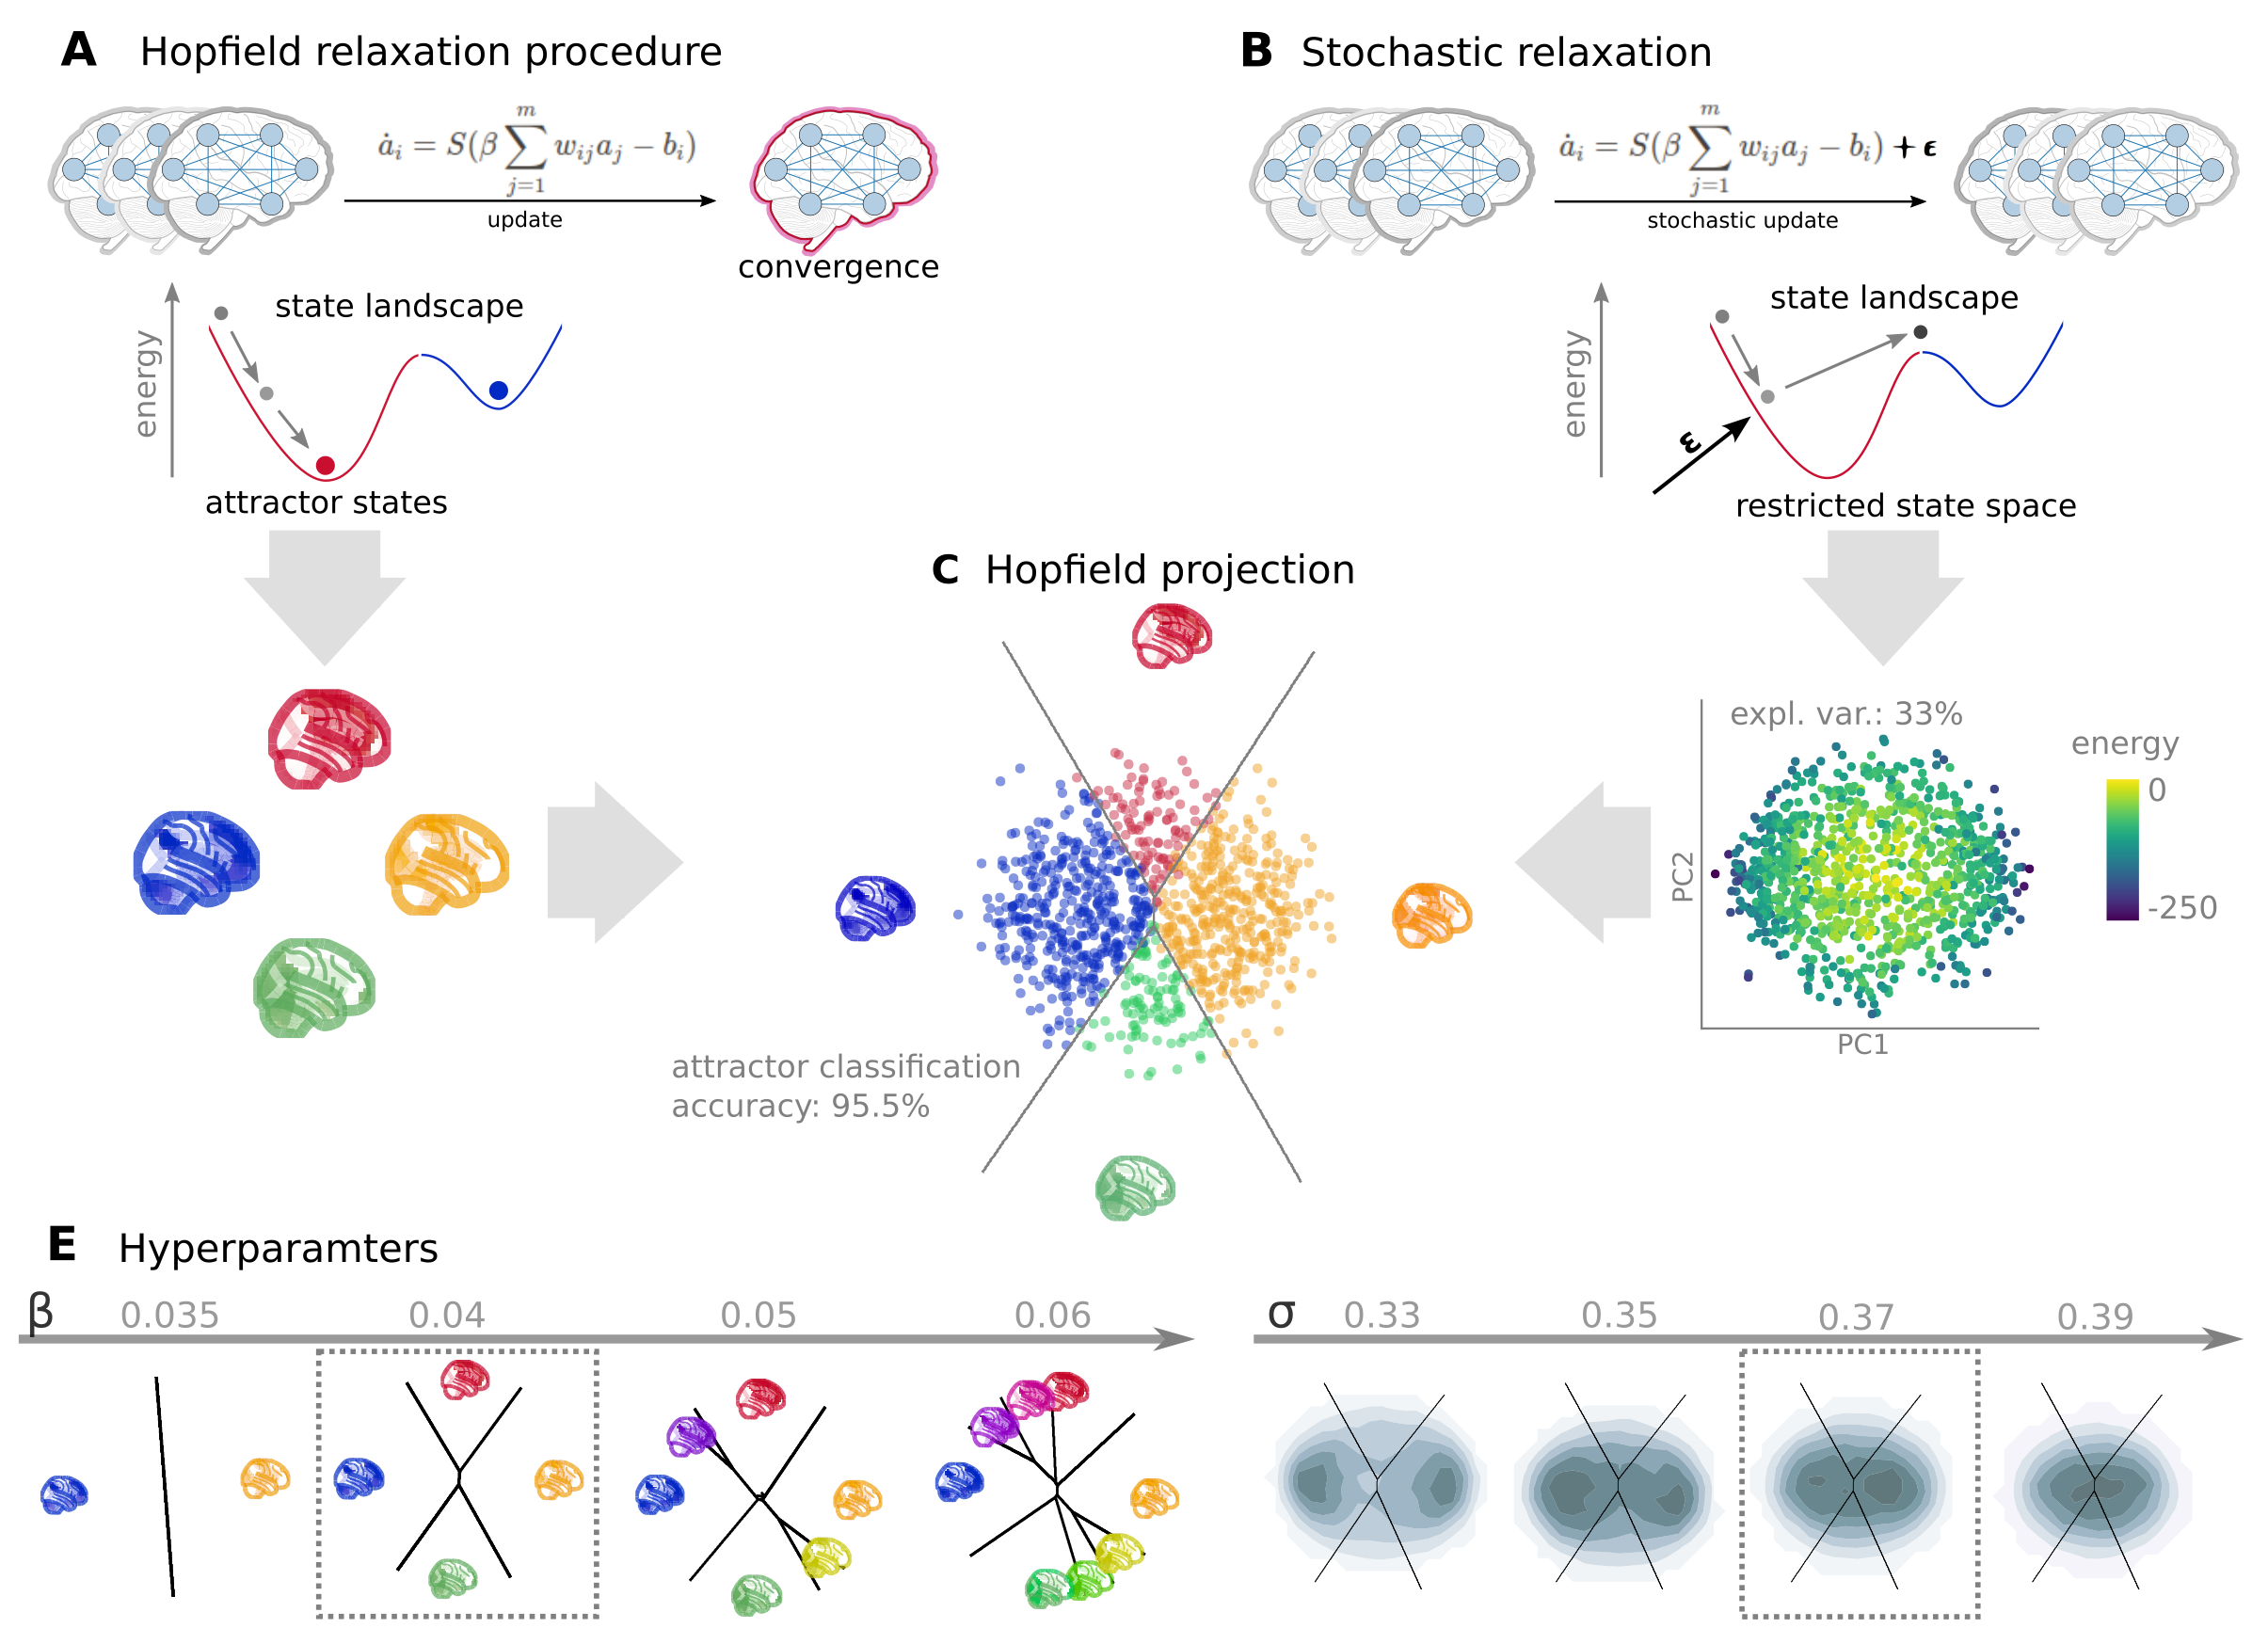
\includegraphics[width=0.7\linewidth]{files/embedding_method-e4ff6c335cd96286e01cc2a26d76ad48.png}
\caption[]{\textbf{Attractor states and state-space dynamics of connectome-based Hopfield networks} \newline
\newline

\textbf{A} Top: During so-called relaxation procedure, activities in the nodes of an \acrshort{fchnn} model are iteratively updated based on the activity of all other regions and the connectivity between them. The energy of a
connectome-based Hopfield network decreases during the relaxation procedure until reaching an equilibrium state with
minimal energy, i.e. an attractor state. Bottom: Four attractor states of the C\acrshort{hnn} derived from the
group-level functional connectivity matrix from Table~\ref{tab-samples} (n=44).
\textbf{B} Top: Similarly to stochastic dynamic causal modeling, in presence of weak noise (stochastic update), the system
does not converge to equilibrium anymore. Instead, activity transverses on the state landscape in a way
restricted by the topology of the connectome and the "gravitational pull" of the attractor states. Bottom: We sample
the state space by running the stochastic relaxation procedure for an extended amount of time (e.g. 100.000 consecutive
stochastic updates), each point representing a possible activation configuration (state). To construct a
low-dimensional representation of the state space, we take the first two principal components of the simulated activity
patterns. The first two principal components explain approximately 58-85\% of the variance of state energy (depending
on the noise parameter $\sigma$, see Figure~\ref{si_expl_variance_energy}).
\textbf{C} We map all states of the state space sample to their corresponding attractor state, with the conventional
Hopfield relaxation procedure (A). The four attractor states are also visualized in their corresponding position on the
PCA-based projection. The first two principal components yield a clear separation of the attractive state basins
(cross-validated classification accuracy: 95.5\%, Figure~\ref{si_classification_acc_state_basins}). We refer to the resulting visualization
as the \acrshort{fchnn} projection and use it to visualize \acrshort{fchnn}-derived and empirical brain dynamics throughout the rest of
the manuscript.
\textbf{E} At its simplest form, the \acrshort{fchnn} framework entails only two free hyperparameters: the temperature parameter
$\beta$ (left) that controls the number of attractor states and the noise parameter of the stochastic relaxation
$\sigma$. To avoid overfitting these parameters to the empirical data, we set $\beta=0.04$ and $\sigma=0.37$ for the
rest of the paper (dotted boxes).}
\label{attractors}
\end{figure}

Consistent with theoretical expectations, we observed that increasing the temperature parameter $\beta$ led to an
increasing number of attractor states (Figure~\ref{attractors}E, left, Figure~\ref{si_att_state_emergence_over_beta}), appearing in symmetric pairs
(i.e. $a_i^{(1)} = -a_i^{(2)}$). For simplicity, we set the temperature parameter for the rest of the paper to a value
resulting in 4 distinct attractor states ($\beta=0.4$).

Fc\acrshort{hnn}s, without any modifications, always converge to an equilibrium state.
To incorporate stochastic fluctuations in neuronal activity \citep{robinson2005multiscale}, we introduced weak
Gaussian noise to the \acrshort{fchnn} relaxation procedure. This procedure, referred to as stochastic relaxation, prevents the system from reaching equilibrium and, somewhat similarly to stochastic DCM \citep{daunizeau2012stochastic}, induces complex system dynamics (Figure~\ref{attractors}B). To sample the resulting state space, we obtained 100,000 iterations of the stochastic relaxation procedure with a Hopfield network initialized with the mean functional connectome in study 1.

In order to enhance interpretability, we generated 100,000 states from the stochastic relaxation procedure in study 1 and obtained the first two principal components of the resulting state space sample.
The resulting two-dimensional embedding (Figure~\ref{attractors}B, bottom plot) exhibited high consistency across different values of $\beta$ and $\sigma$ (Figure~\ref{attractors}E).
For all subsequent analyses, we set \${\textbackslash}sigma=0.37 (based a coarse optimization procedure aimed at reconstructing the bimodal distribution of empirical data, Figure~\ref{attractors}E right). On the low-dimensional embedding, which we refer to as the \textit{\acrshort{fchnn} projection}, we observed a clear separation of the attractor states (Figure~\ref{attractors}C), with the two symmetric pairs of attractor states located at the extremes of the first and second PC.
To map the attractor basins on the space spanned by the first two PCs (Figure~\ref{attractors}C), we obtained the attractor state of each point visited during the stochastic relaxation and fit a multinomial logistic regression model to predict the attractor state from the first two PCs.
The resulting model accurately predicted attractor states of arbitrary brain activity patterns, achieving a cross-validated accuracy of 96.5\%.
The attractor basins were visualized by using the decision boundaries obtained from this model. (Figure~\ref{attractors}C). We propose the 2-dimensional \acrshort{fchnn} projection depicted on (Figure~\ref{attractors}C) as a simplified representation of brain dynamics, and use it as a basis for all subsequent analyses in this work. Examples are presented on Figure~\ref{example-trajectories}.

\begin{figure}[!htbp]
\centering
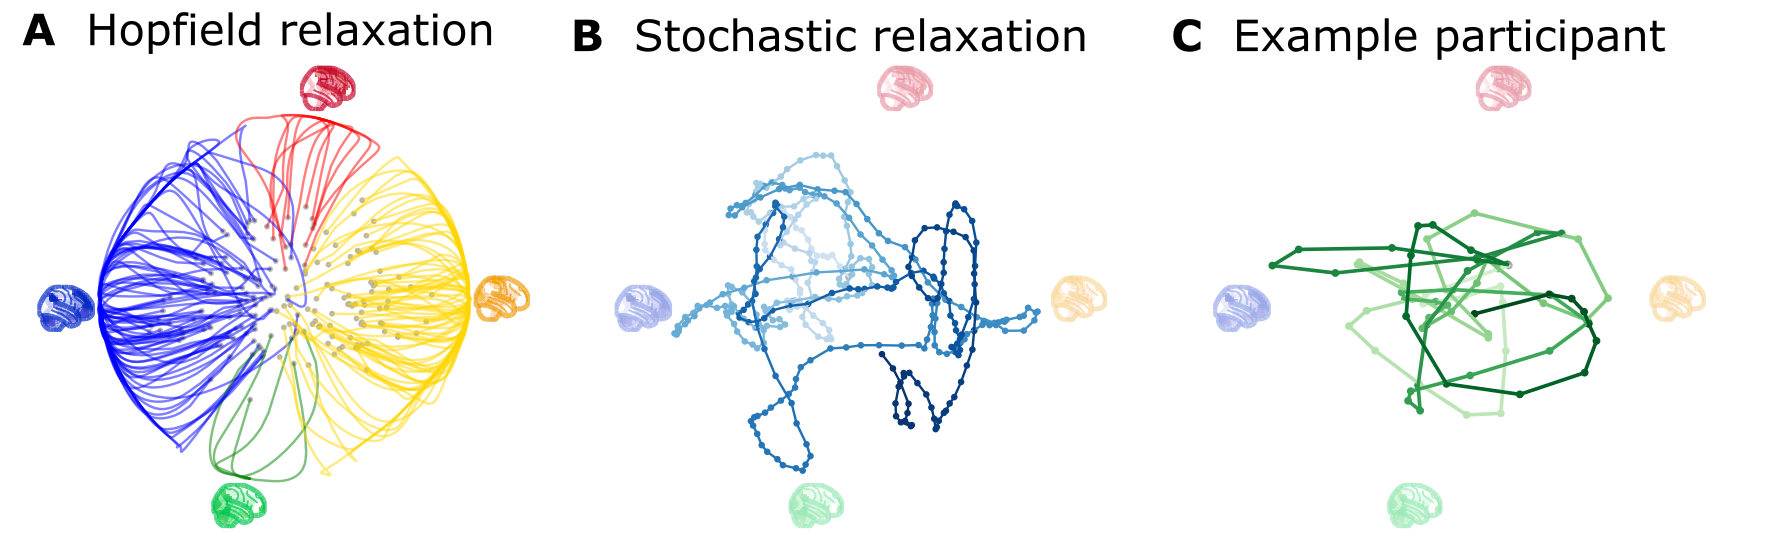
\includegraphics[width=0.7\linewidth]{files/trajectories-07527e4626d2523997c92ea93bb32054.png}
\caption[]{\textbf{Examples trajectories on the \acrshort{fchnn} projection.}\newline
\newline

\textbf{A} The \acrshort{fchnn} of study 1 seeded with real activation maps (gray dots) of an example participant. All activation maps converge to one of the four attractor states during the relaxation procedure (without noise). Trajectories are colored by attractor state.
\textbf{B} Illustration of the stochastic relaxation procedure in the same \acrshort{fchnn} model. The system does not converge to an attractor state but instead transverses the state space in a way restricted by the topology of the connectome and the "gravitational pull" of the attractor states. The shade of the trajectory changes with increasing number of iterations. The trajectory is smoothed with a moving average over 10 iterations for visualization purposes.
\textbf{C} Real resting state \acrshort{fmri} data of an example participant from study 1, plotted on the \acrshort{fchnn} projection. The shade of the trajectory changes with increasing number of iterations.}
\label{example-trajectories}
\end{figure}

\subsubsection{Reconstruction of resting state brain dynamics}

The spatial patterns of the obtained attractor states exhibit high neuroscientific relevance and closely resemble previously described large-scale brain systems. (Figure~\ref{rest-validity}A). The first pair of attractors (mapped on PC1, horizontal axis) resemble the two complementary ``macro'' systems described, among others, by \citet{golland2008data} and \citet{cioli2014differences} as well as the two "primary" brain states observed by \citet{chen2018human} and the 'unimodal to transmodal' principal gradient of \citet{margulies2016situating} and \citet{huntenburg2018large}. A common interpretation of these two patterns is that they represent (i) an ``extrinsic'' system which exhibits a stronger direct connection to the immediate sensory environment and (ii) an "intrinsic" system, whose activity is primarily associated with dynamic changes in higher-level internal context and closely linked to the default mode network.
The other pair of attractors spans an orthogonal axis, and resemble to patterns commonly associated with perception--action cycles \citep{fuster2004upper}, and described as a gradient across sensory-motor modalities \citep{huntenburg2018large}, recruiting regions associated with active inference (e.g. motor cortices) and perceptual inference (e.g visual areas).

\begin{figure}[!htbp]
\centering
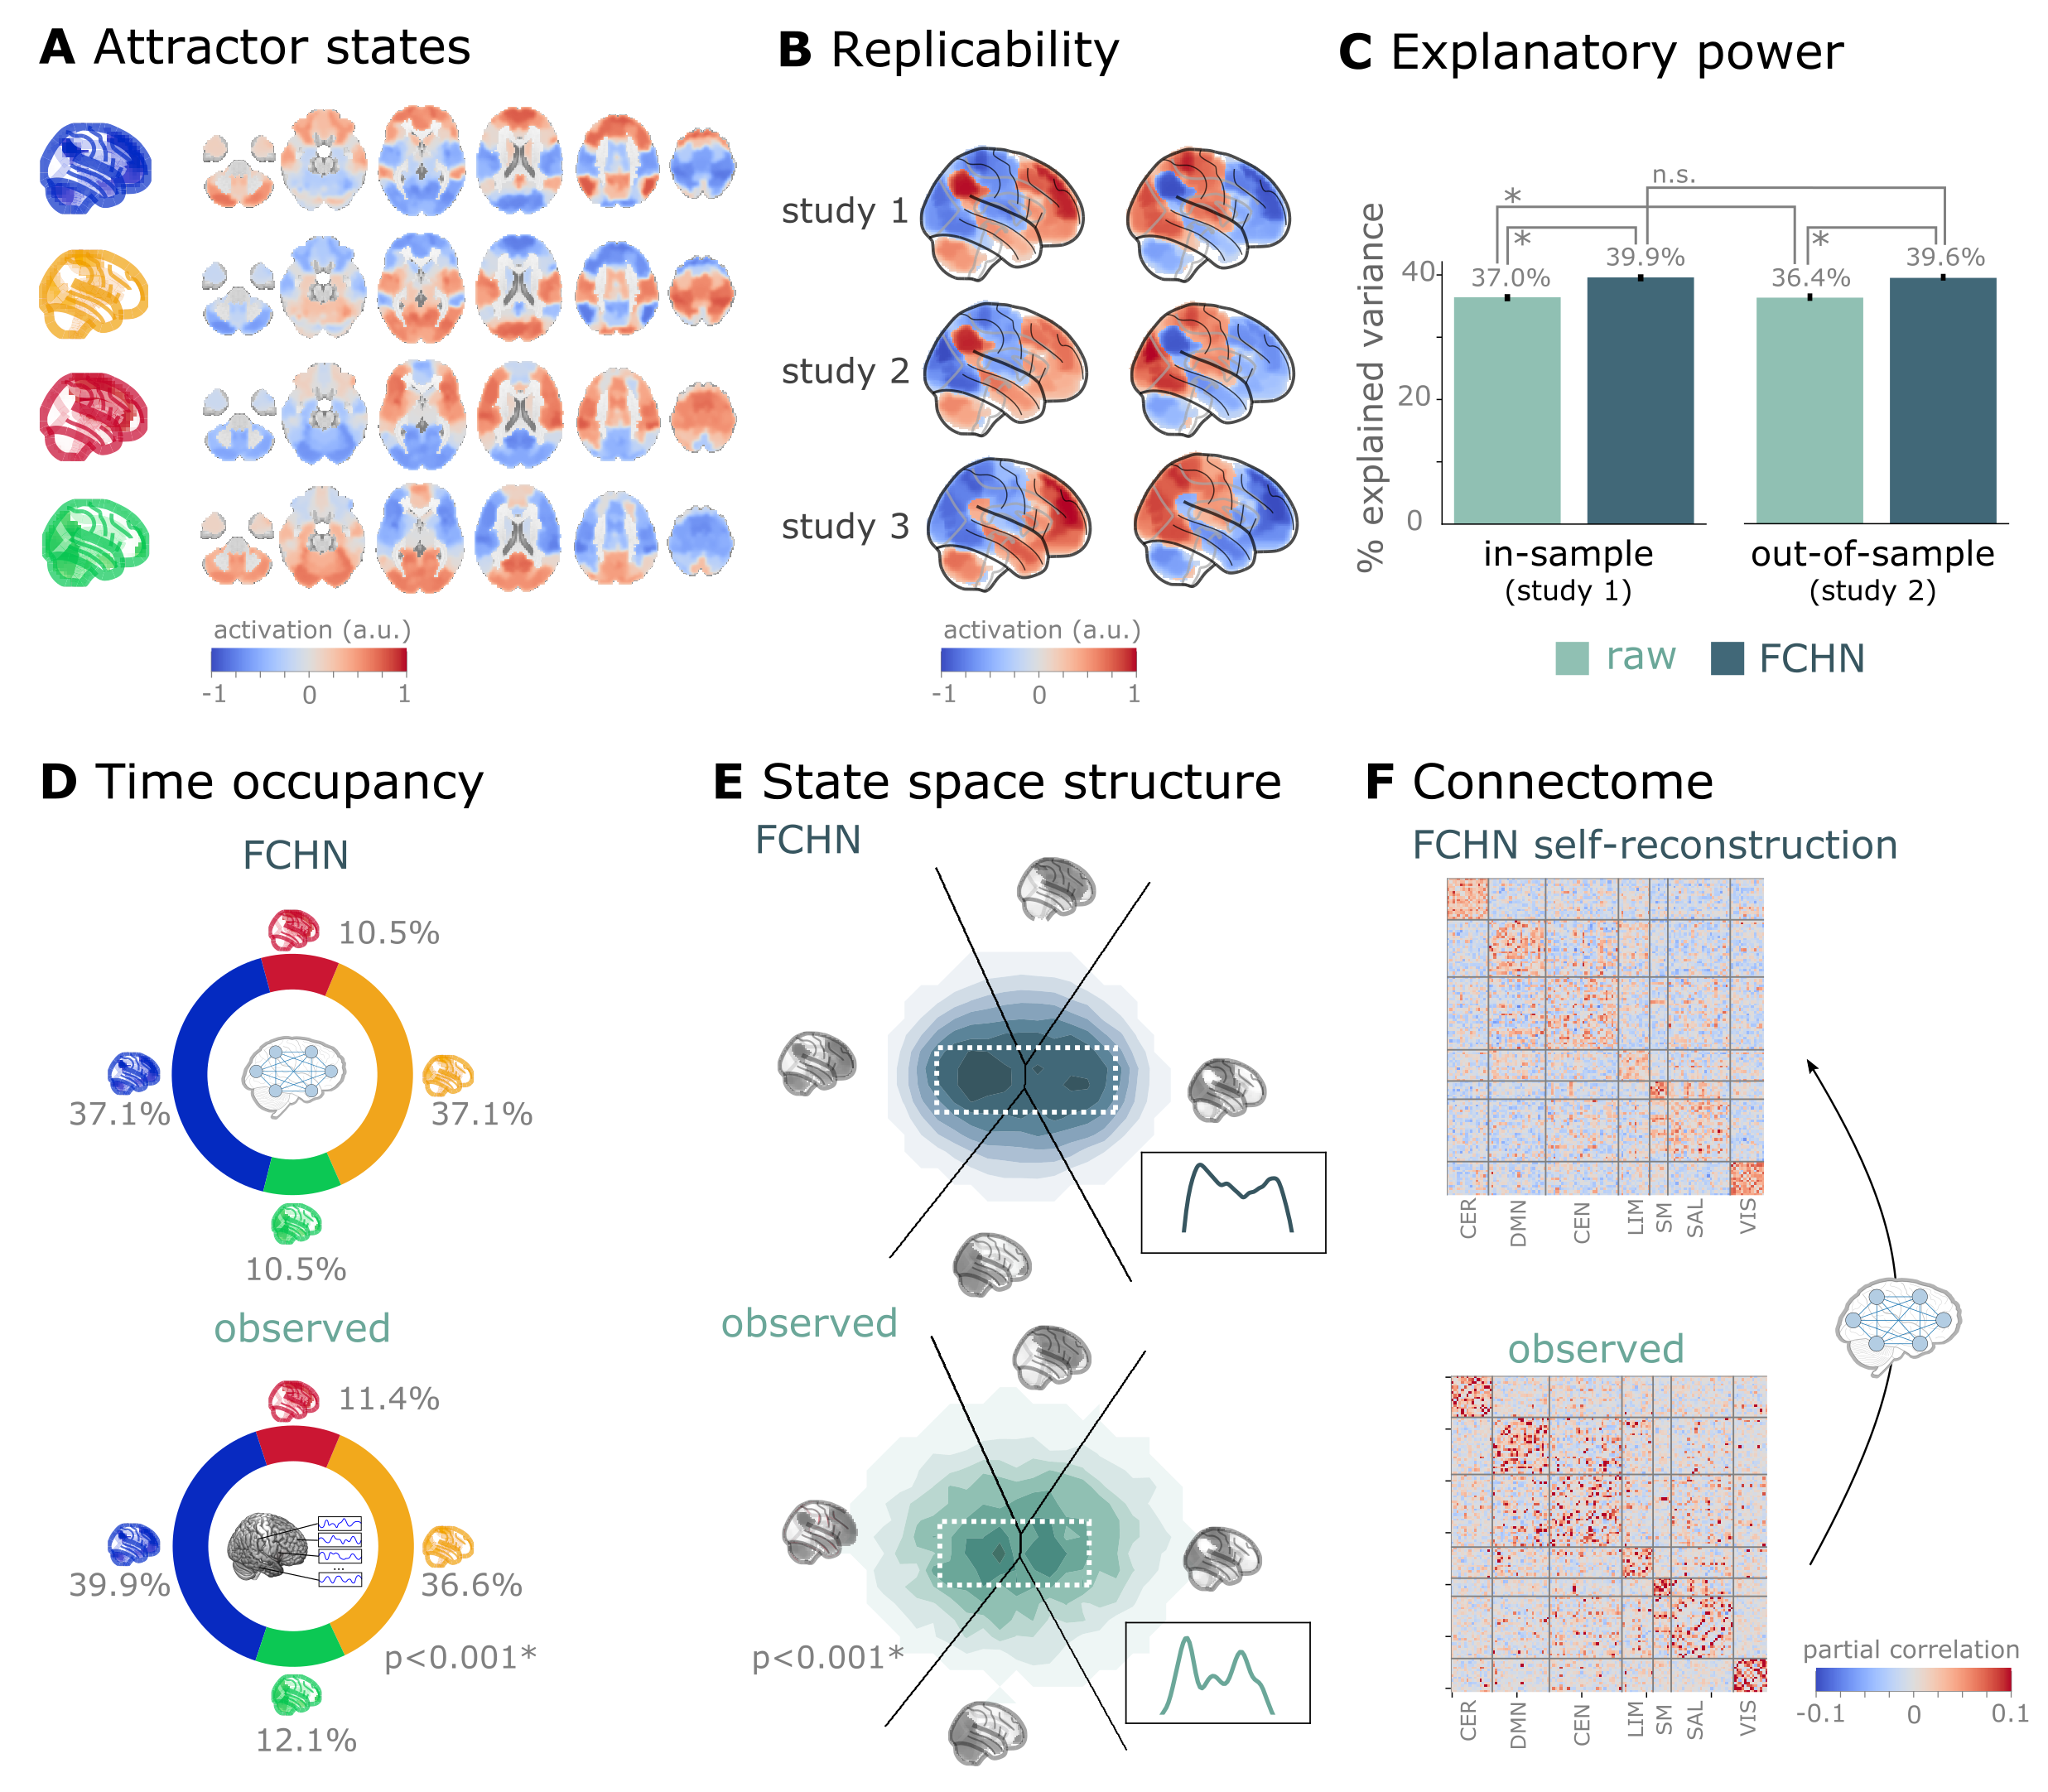
\includegraphics[width=0.7\linewidth]{files/face_validity-7322409cd26e6c076f9869fd7895a11f.png}
\caption[]{\textbf{Connectome-based Hopfield networks reconstruct characteristics of real resting state brain activity.}\newline
\newline

\textbf{A} The four attractor states of the \acrshort{fchnn} model from study 1 reflect brain activation
patterns with high neuroscientific relevance, representing sub-systems previously associated with 'internal context'
(blue), "external context" (yellow), "action/execution" (red) and "perception" (green)
\citep{golland2008data, cioli2014differences, chen2018human, fuster2004upper, margulies2016situating}.
\textbf{B} The attractor states show excellent replicability in two external datasets (study 2 and 3, mean correlation 0.93).
\textbf{C} The \acrshort{fchnn} projection (first two PCs of the \acrshort{fchnn} state space) explains significantly more variance (p\textless 0.0001) in the real
resting state \acrshort{fmri} data than principal components derived from the real resting state data itself and generalizes
better (p\textless 0.0001) to out-of-sample data (study 2). Error bars denote 99\% bootstrapped confidence intervals.
\textbf{D} The \acrshort{fchnn} analysis accurately predicts (p\textless 0.0001) the fraction of time spent on the basis of the four attractor
states in real restring state \acrshort{fmri} data (study 1) and,
\textbf{E}, reconstructs the characteristic bimodal distribution of the real resting state data.
\textbf{F} Stochastic \acrshort{fchnn}s are capable of self-reconstruction: the timeseries resulting from the stochastic relaxation procedure
mirror the co-variance structure of the functional connectome the \acrshort{fchnn} model was initialized with.}
\label{rest-validity}
\end{figure}

Importantly, the discovered attractor states demonstrate a remarkable level of replicability (mean Pearson's
correlation 0.93) across the discovery datasets (study 1) and two independent replication datasets
(Table~\ref{tab-samples}, Figure~\ref{rest-validity}C) and robust to noise added to the connectome (\{numref\}`Supplementary Figure \%s \textless si\_noise\_robustness\_weights\textgreater ).

Further analysis in study 1 showed that connectome-based Hopfield models accurately reconstructed multiple
characteristics of true resting-state data.

First, the first two components of the \acrshort{fchnn} projection accounted for a substantial amount of variance in the real resting-state \acrshort{fmri} data in study 1 (mean $R^2=0.399$) and generalized well to out-of-sample data (study 2, mean $R^2=0.396$)  (Figure~\ref{rest-validity}E). Remarkably, the explained variance of the \acrshort{fchnn} projection significantly exceeded that of a PCA performed directly on the real resting-state \acrshort{fmri} data itself ($R^2=0.37$ and $0.364$ for in- and out-of-sample analyses).

Second, \acrshort{fchnn} analyses accurately reconstructed true resting state brain state dynamics. During stochastic relaxation, the \acrshort{fchnn} model was found to spend approximately three-quarters of the time on the basis of the first two attractor states, with an equal distribution between them. The remaining one-quarter of the time is spent on the basis of the second pair of attractor states, also equally distributed. We observed strikingly similar temporal occupancies in the real data Figure~\ref{rest-validity}D), statistically significant with various null models (Figure~\ref{si_state_occcupancy_null_models}). Not onyl state occupancies, but fine-grained details of the bimodal distribution observed in the real resting-state \acrshort{fmri} data were also convincingly reproduced by the \acrshort{fchnn} model (Figure~\ref{rest-validity}F and Figure~\ref{attractors}E).

Finally, \acrshort{fchnn}s were found to generate signal that preserves the covariance structure of the real functional connectome, indicating that dynamic systems of this type (inclusing the brain) inevitably "leak" their underlying structure into the activity time series, strengthening the construct validity of our approach (Figure~\ref{rest-validity}D).

\subsubsection{An explanatory framework for task-based brain activity}

Next to reproducing various characteristics of spontaneous brain dynamics, \acrshort{fchnn}s can also be used to model responses to various perturbations. We obtained task-based \acrshort{fmri} data from a study by \citet{woo2015distinct} (Table~\ref{tab-samples}, n=33, see Figure~\ref{rest-validity}), investigating the neural correlates of pain and its self-regulation.
We found that activity changes due to pain (taking into account hemodynamics, see Methods) were characterized on the \acrshort{fchnn} propjection by a shift towards the attractor state of action/execution (permutation test for mean projection difference by randomly swapping conditions, p\textless 0.001, Figure~\ref{task-validity}A, left). Energies, as defined by the \acrshort{hnn}, were also significantly different between the two conditions (p\textless 0.001), with higher energies during pain stimulation.

When participants were instructed to up- or down-regulate their pain sensation (resulting in increased and decreased pain reports and differential brain activity in the nucleus accumbens, NAc (see \cite{woo2015distinct} for details), we observed further changes of the location of momentary brain activity patterns on the \acrshort{fchnn} projection (p\textless 0.001, Figure~\ref{task-validity}A, right), with down-regulation pulling brain dynamics towards the attractor state of internal context. Interestingly, self-regulation did not trigger significant energy changes (p=0.36).

\begin{figure}[!htbp]
\centering
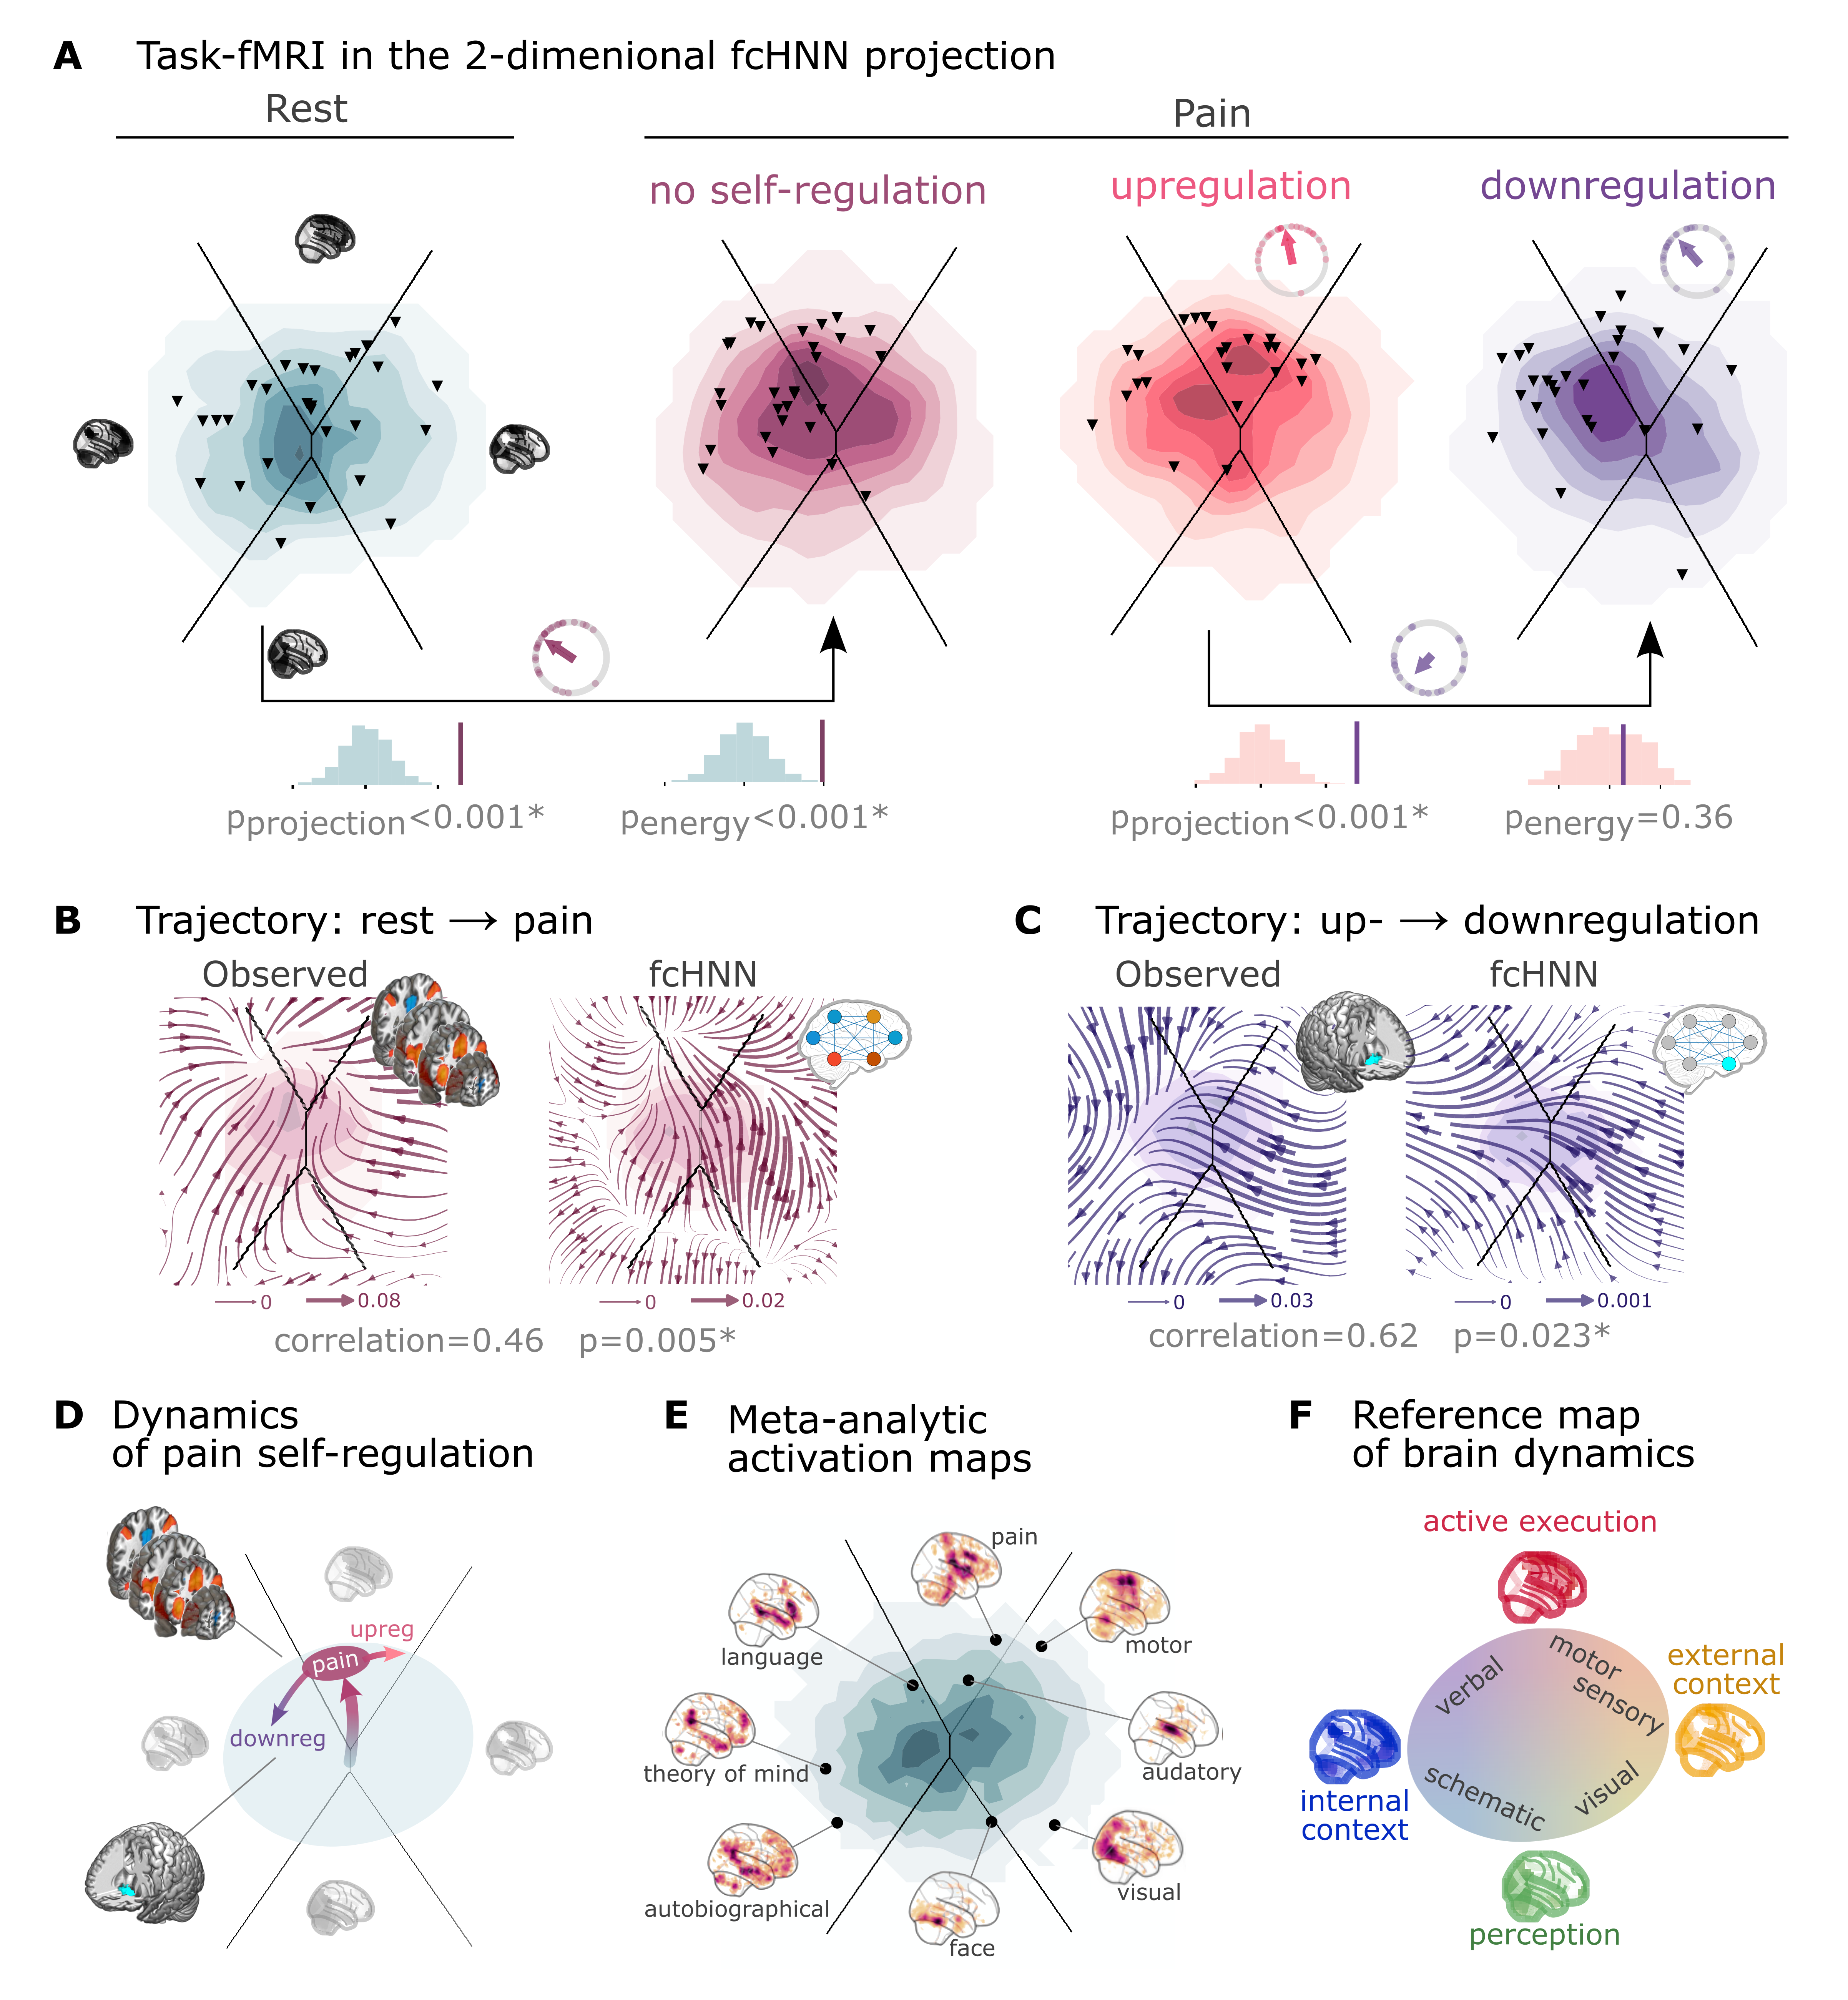
\includegraphics[width=0.7\linewidth]{files/task_validity-706d1e22910e17771562c2d5ef3a4928.png}
\caption[]{\textbf{Empirical Hopfield-networks reconstruct real task-based brain activity.} \newline

\textbf{A} Functional MRI time-frames during pain stimulation from Table~\ref{tab-samples} (second \acrshort{fchnn} projection plot)
and self-regulation (third and fourth) are distributed differently on the \acrshort{fchnn} projection than brain states
during rest (first projection, permutation test, p\textless 0.001 for all). Energies, as defined by the Hopfield model, are also
significantly different between rest and the pain conditions (permutation test, p\textless 0.001), with higher energies during
pain stimulation. Triangles denote participant-level mean activations in the various blocks (corrected for
hemodynamics). Small circle plots show the directions of the change for each individual (points) as well as the mean direction
across participants (arrow), as compared to the reference state (downregulation for the last circle plot, rest for all
other circle plots).
\textbf{B} Flow-analysis (difference in the average timeframe-to-timeframe transition direction) reveals a non-linear difference in brain dynamics during pain and rest (left). When introducing weak pain-related signal in the \acrshort{fchnn} model during stochastic relaxation, it accurately reproduces these non-linear flow differences (right).
\textbf{C} Simulating activity in the Nucleus Accumbens (NAc) (the region showing significant activity differences in \cite{woo2015distinct}) reconstructs the observed non-linear flow difference between up- and downregulation (left).
\textbf{D} Schematic representation of brain dynamics during pain and its up- and downregulation, visualized on the \acrshort{fchnn}  projection. In the proposed framework, pain does not simply elicit a direct response in certain regions, but instead, shifts spontaneous brain dynamics towards the "action" attractor, converging to a characteristic "ghost attractor" of pain. Down-regulation by NAc activation exerts force towards the attractor of internal context, leading to the brain less frequent "visiting" pain-associated states.
\textbf{E} Visualizing meta-analytic activation maps on the \acrshort{fchnn} projection captures intimate relations between the corresponding tasks and \textbf{F} serves as a basis for a \acrshort{fchnn}-based theoretical interpretative framework for spontaneous and task-based brain dynamics. In the proposed framework, task-based activity is not a mere response to external stimuli in certain brain locations but a perturbation of the brain's characteristic dynamic trajectories, constrained by the underlying functional connectivity. From this perspective, "activity maps" from conventional task-based \acrshort{fmri} analyses capture time-averaged differences in these whole brain dynamics.}
\label{task-validity}
\end{figure}

Next, we conducted a "flow analysis" on the \acrshort{fchnn} projection, quantifying how the average timeframe-to-timeframe transition direction differs on the \acrshort{fchnn} projection between conditions (see Methods).
This analysis unveiled that during pain (Figure~\ref{task-validity}B, left side), brain activity tends to gravitate towards a distinct point on the projection, which we term the "ghost attractor" of pain (similar to \cite{vohryzek2020ghost}). In terms of attractor states, this belongs to the basin of the attractor corresponding to action/execution. In case of downregulation (as compared to upregulaion), brain activity is pulled away from the pain-related "ghost attractor" (Figure~\ref{task-validity}C, left side), towards the attractor of internal context.

Functional connectivity-based \acrshort{hnn}s were able to accurately reconstruct these non-linear dynamics by adding a small amount of realistic "control signal" (similarly to network control theory \citet{liu2011controllability, gu2015controllability}). To simulate the alterations in brain dynamics during pain stimulation, we acquired a meta-analytic pain activation map \citep{zunhammer2021meta} (n=603) and incorporated it as additional signal, along with the Gaussian noise, during the stochastic relaxation procedure. The ghost attractor found in the empirical data was present with signal-to-noise (SNR) values ranging from 0.003 to 0.009 (), we found that by adding a minimal amount of signal (SNR = 0.005), the \acrshort{fchnn} model achieved a remarkable reconstruction of the observed non-linear disparities in brain dynamics between the pain and rest conditions, including the characteristic pain-related "ghost attractor". (Pearson's r = 0.46, p=0.005 when randomizing conditions on a per-participant basis, Figure~\ref{task-validity}B, right side).

The same model was also able to reconstruct the observed non-linear differences in brain dynamics between the up- and downregulation conditions (Pearson's r = 0.62, p=0.023) without any further optimization (SNR=0.005,
Figure~\ref{task-validity}C, right side). The only change we made to the model was the addition (downregulation) or
subtraction (upregulation) of control signal in the NAc (the region in which \citep{woo2015distinct} observed significant changes between up- and downregulation), introducing a signal difference of $Delta$ SNR=0.005 (the same we found optimal in the previous analysis). Results were reproducible with lower NAc SNRs, too (Figure~\ref{si_downreg_trajectory_sim}).

To provide a comprehensive picture on how tasks and stimuli other then pain map onto the \acrshort{fchnn} projection, we obtained various task-based meta-analytic activation maps from Neurosynth (see Methods) and plotted them on the \acrshort{fchnn} projection (Figure~\ref{task-validity}E). This analysis reinforced and extended our interpretation of the four investigated attractor states and shed more light on how various functions are mapped on the axes of internal vs. external context and perception vs. action.
In the coordinate system of the \acrshort{fchnn} projection, visual processing is labeled "external-perception", sensory-motor processes "external-active", language, verbal cognition and working memory is labelled "internal-active" and long-term memory as well as social and autobiographic schemata fall into the "internal-perception" regime (Figure~\ref{task-validity}F).

\subsubsection{Clinical relevance}

We obtained data from n=172 individuals acquired at the New York University Langone Medical Center, New York, NY, USA (NYU) as shared in the Autism Brain Imaging Data Exchange dataset (Table~\ref{tab-samples}: \acrshort{abide}, \citep{di2014autism}.
After excluding high-motion cases (see Methods), we visualized the distribution of time-frames on the \acrshort{fchnn}-projection separately for \acrshort{asd} patients and typically developing control (TDC) participants (Figure~\ref{clinical-validity}A).
We found several significant differences in the mean attractor activation (see Methods) in the \acrshort{asd} group as compared to the respective controls (Figure~\ref{clinical-validity}B).
Strongest differences were found on the "action-perception" axis (Table~\ref{tab-clinical-results}), with increased activity of the sensory-motor and mid\acrshort{dl}e cingular cortices during "action-execution" related states and increased visual and decreased sensory and auditory activity during "perception" states, likely reflecting the widely acknowledged, yet poorly understood, perceptual atypicalities in \acrshort{asd} \citep{hadad2019perception}. \acrshort{asd} related changes in the internal-external axis were characterized by more involvement of the posterior cingulate, the precuneus, the nucleus accumbens, the dorsolateral prefrontal cortex (\acrshort{dl}\acrshort{pfc}), the cerebellum (Crus II, lobule VII) and inferior temporal regions during activity of the internalizing subsystem (Table~\ref{tab-clinical-results}). While similar, default mode network (DMN)-related changes have often been attributed to an atypical integration of information about the ``self'' and the ``other'' \citep{padmanabhan2017default}, a more detailed \acrshort{fchnn}-analysis may help to further disentangle the specific nature of these changes.

\begin{figure}[!htbp]
\centering
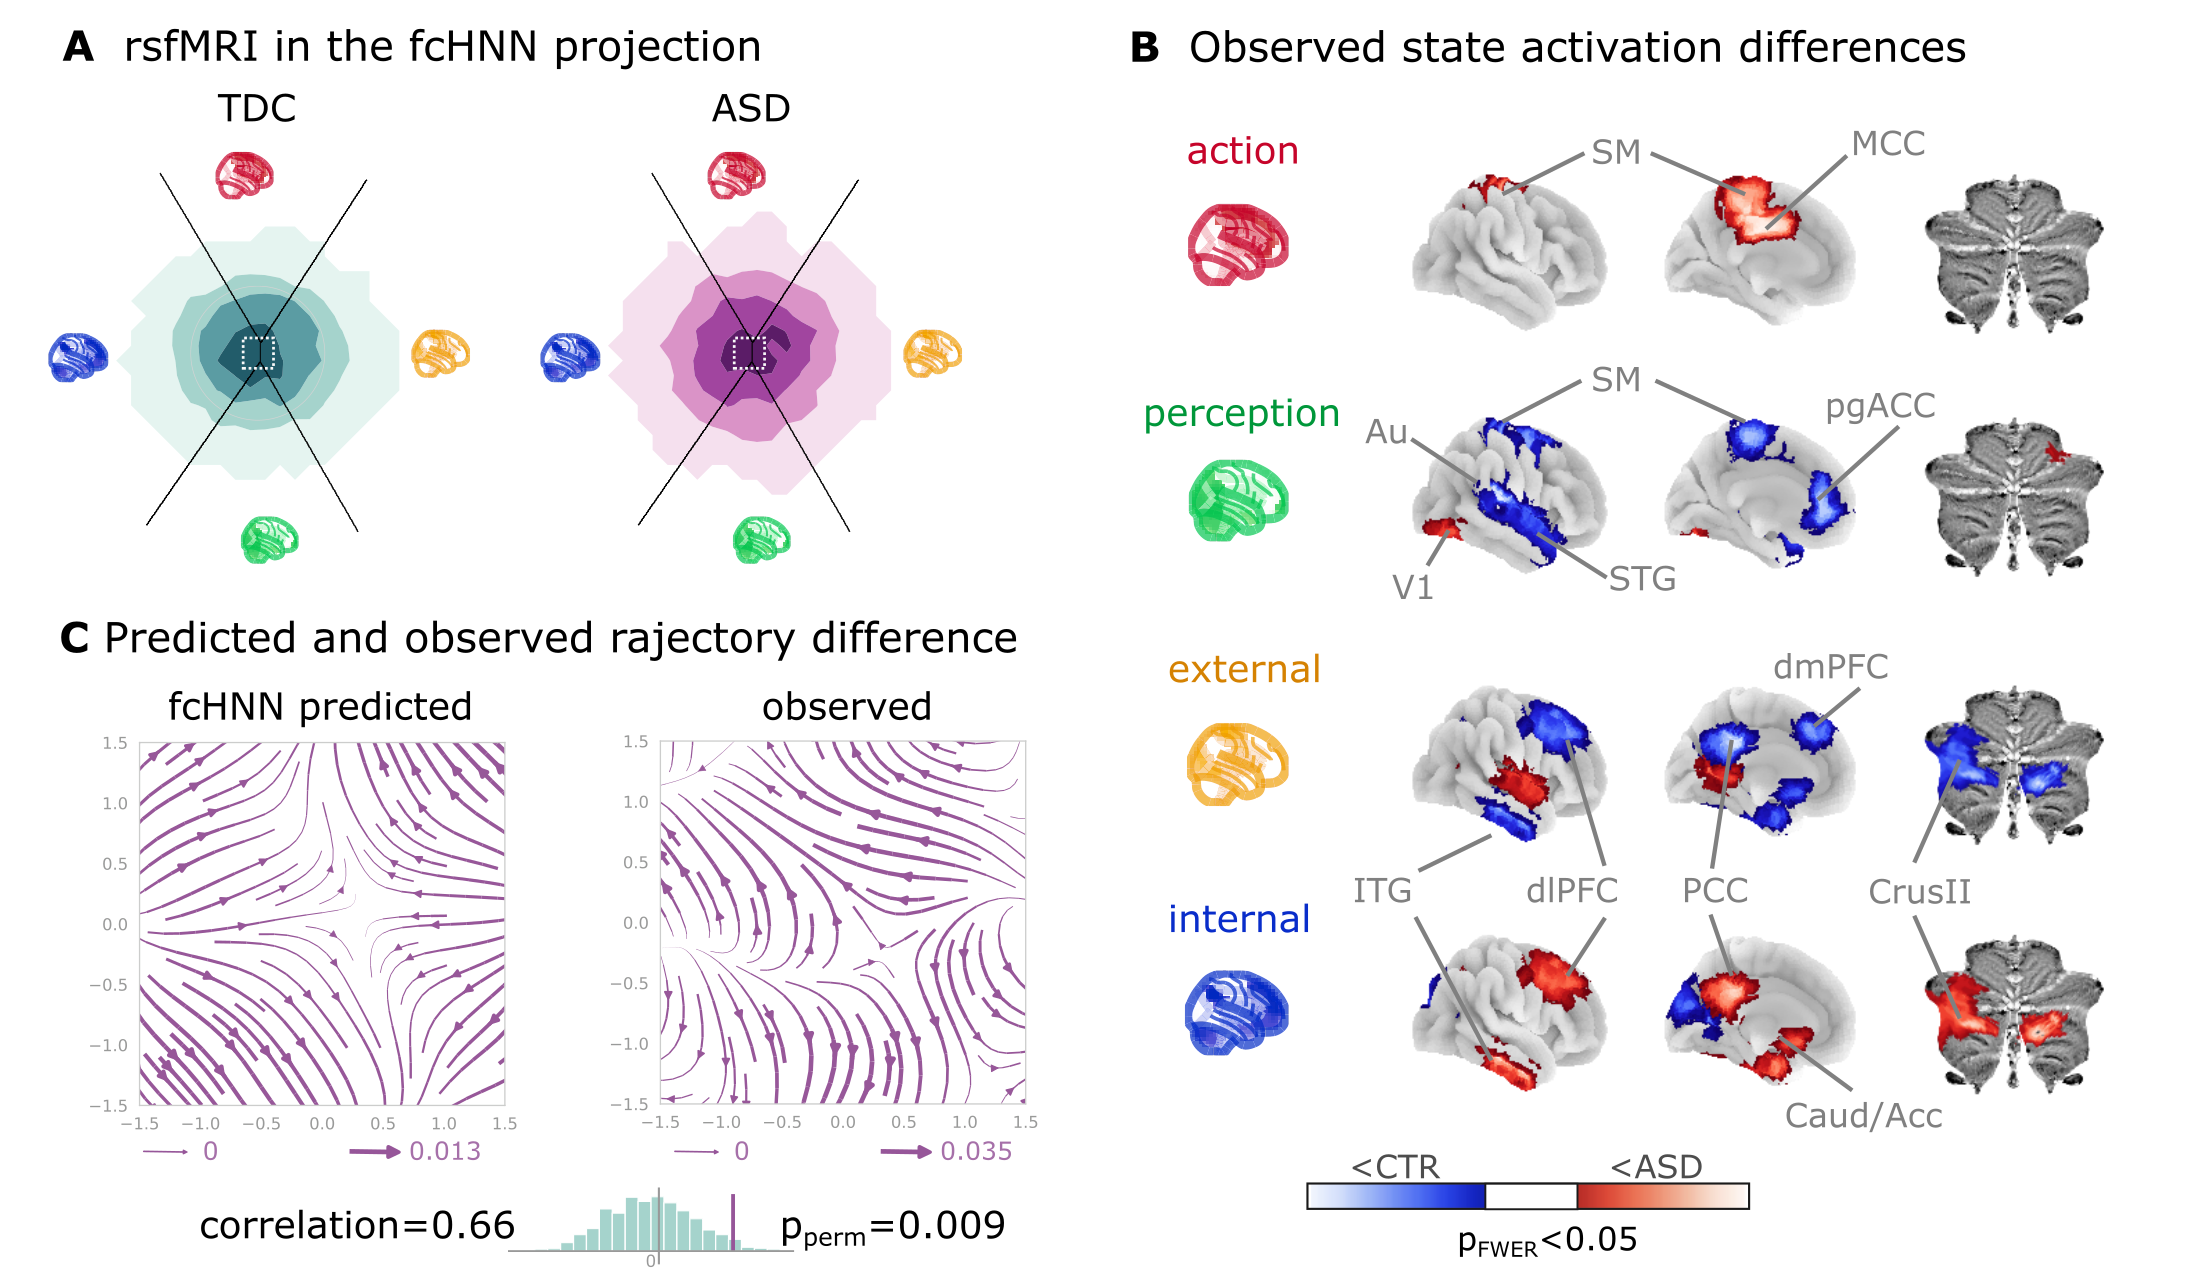
\includegraphics[width=0.7\linewidth]{files/state_analysis-ceb6decce59475025731579acd14f1ec.png}
\caption[]{\textbf{Connectome-based Hopfield analysis of autism spectrum disorder.} \newline

\textbf{A} The distribution of time-frames on the \acrshort{fchnn}-projection separately for \acrshort{asd} patients and typically developing control (TDC) participants. \newline

\textbf{B} We quantified attractor state activations in the Autism Brain Imaging Data Exchange datasets (Table~\ref{tab-samples}) as the
individual-level mean activation of all time-frames belonging to the same attractor state. This analysis captured alterations similar to those previously associated to \acrshort{asd}-related perceptual atypicalities (visual, auditory and somatosensory cotices) as well as atypical integration of information about the ``self'' and the ``other'' (default mode network regions). All results are corrected for multiple comparisons across brain regions and attractor states (122*4 comparisons) with Bonferroni-correction. See Table~\ref{tab-clinical-results} and Figure~\ref{si_clinical_results_table} for detailed results. \newline

\textbf{C} The comparison of data generated by \acrshort{fchnn}s initilaizeed with \acrshort{asd} and TDC cconnectomes, respectively, revealed a characteristic pattern of differences in the system's dynamics, with increased pull towards (and potentially a higher separation between) the action and perception attractors attractors and a lower tendency of trajectories going towards the internal and external attractors. \newline

\textit{\textbf{Abbreviations}: \acrshort{mcc}: mid\acrshort{dl}e cingulate cortex, \acrshort{acc}: anterior cingulate cortex, \acrshort{pg}: perigenual, \acrshort{pfc}: prefrontal cortex, \acrshort{dm}: dorsomedial, \acrshort{dl}: dorsolateral, \acrshort{stg}: superior temporal gyrus, \acrshort{itg}: inferior temporal gyrus, \acrshort{caud/acc}: caudate-accumbens,  \acrshort{sm}: sensorimotor, \acrshort{v1}: primary visual, \acrshort{a1}: primary auditory, \acrshort{sm}A: supplementary motor cortex, \acrshort{asd}: autism spectrum disorder, TDC: typically developing control.}}
\label{clinical-validity}
\end{figure}

\begin{table}
\centering
\caption[]{\textbf{The top ten largest changes in average attractor-state activity beetween autistic and control individuals.}  Mean attractor-state activity changes are presented in the order of their absolute effect size. All p-values are based on permutation tests (shuffling the group assignment) and corrected for multiple comparisons (via Bonferroni's correction). For a comprehensive list of significant findings, see \{numref\}`Supplementary Figure \%s \textless si\_clinical\_results\_table\textgreater .}
\label{tab-clinical-results}
\begin{tabular}{p{\dimexpr 0.250\linewidth-2\tabcolsep}p{\dimexpr 0.250\linewidth-2\tabcolsep}p{\dimexpr 0.250\linewidth-2\tabcolsep}p{\dimexpr 0.250\linewidth-2\tabcolsep}}
\toprule
region & attractor & effect size & p-value \\
\hline
primary auditory cortex & perception & -0.126 & \textless 0.0001 \\
mid\acrshort{dl}e cingulate cortex & action & 0.109 & \textless 0.0001 \\
cerebellum lobule VIIb (medial part  ) & internal context & 0.104 & \textless 0.0001 \\
mediolateral sensorimotor cortex & perception & -0.099 & 0.00976 \\
precuneus & action & 0.098 & \textless 0.0001 \\
mid\acrshort{dl}e superior temporal gyrus & perception & -0.098 & \textless 0.0001 \\
frontal eye field & perception & -0.095 & \textless 0.0001 \\
dorsolateral sensorimotor cortex & perception & -0.094 & 0.00976 \\
posterior cingulate cortex & action & 0.092 & \textless 0.0001 \\
dorsolateral prefrontal cortex & external context & -0.092 & \textless 0.0001 \\
\bottomrule
\end{tabular}
\end{table}

Thus, we contrasted the characteristic trajectories derived from the \acrshort{fchnn} models of the two groups (initialized with the group-level functional connectomes). Fc\acrshort{hnn} modelling predicted that in \acrshort{asd}, there is an increased likelihood of states returning towards the mid\acrshort{dl}e from the internal-external axis and an increased likelihood of states transitioning towards the extremes of the action-perception axis (Figure~\ref{clinical-validity}C). We observed a highly similar pattern in the real data (Pearson's correlation: 0.66), statistically significant after permutation testing (shuffling the group assignment, p=0.009).

\subsection{Discussion}

In this study, we have introduced and validated a simple yet robust computational generative framework that elucidates how activity propagation within the functional connectome orchestrates large-scale brain dynamics, leading to the spontaneous emergence of brain states and characteristic dynamic responses to perturbations.
The construct validity of our model is rooted in the activity flow principle, first introduced by \citet{cole2016activity}. The activity flow principle states that activity in a brain region can be predicted by a weighted combination of the activity of all other regions, where the weights are set to the functional connectivity of those regions to the held-out region. This principle has been shown to hold across a wide range of experimental and clinical conditions \citep{cole2016activity, ito2017cognitive, mill2022network, hearne2021activity, chen2018human}.
The proposed approach is based on the intuition that the repeated, iterative application of the activity flow equation in a system exhibits close analogies with a type of recurrent artificial neural networks known as Hopfield networks \citep{hopfield1982neural}.

Hopfield networks have previously been shown to exhibit a series of characteristics that are also highly relevant for
brain function, including the ability to store and recall memories \citep{hopfield1982neural}, self-repair \citep{murre2003selfreparing},
a staggering robustness to noisy or corrupted inputs \citep{hertz1991introduction} (see also Figure~\ref{si_noise_robustness_weights}) and the ability to produce multistable dynamics organized by the "gravitational pull" of a finite number of attractor states \citep{khona2022attractor}. While many of such properties of Hopfield networks have previously been proposed as a model for micro-scale neural systems (see \cite{khona2022attractor} for a review), the proposed link between macro-scale activity propagation and Hopfield networks allows transferring the vast body of knowledge on Hopfield networks to the study of large-scale brain dynamics.

Integrating Cole's activity flow principle with the \acrshort{hnn} architecture mandates the initiation of network weights with functional connectivity values, specifically partial correlations as suggested by \citet{cole2016activity}.
Considering the functional connectome as weights of an already trained neural network distinguishes our methodology not only from conventional biophysical and phenomenological computational modeling strategies, which usually rely on the structural connectome as a proxy for polysynaptic connectivity \citep{cabral2017functional}, but also from "neuroconnectionist" approaches that employ explicit training procedures \citep{doerig2023neuroconnectionist}.

As compared to finely detailed biophysical models with many free parameters, the basic form of the \acrshort{fchnn} approach comprises solely two "hyperparameters" (temperature and noise) and yields notably consistent outcomes across an extensive range of these parameters (Figure~\ref{si_expl_variance_energy}, Figure~\ref{si_att_state_emergence_over_beta}, Figure~\ref{si_state_occcupancy_null_models}, Figure~\ref{si_pain_ghost_attractor_sim}, Figure~\ref{si_downreg_trajectory_sim})). To underscore the potency of this simplicity and stability, in the present work, we avoided any unneccessary parameter optimization.

Another advantage of fC\acrshort{hnn}s over more detailed models ias that \acrshort{fchnn}s are relativela easy to interpret as they establish a direct link between two highly prevalent metrics of brain function: functional connectivity and brain activity. This connection is not solely phenomenological, but also mathematical, facilitating the exploration and prediction of alterations in the system's dynamics in response to perturbations affecting both activity and connectivity.

The proposed model also exhibits several advantages over linear network control theory-based \citep{gu2015controllability} approaches. First, the \acrshort{fchnn} approach works with direct activity flow estimates and does not require knowledge about the structural-functional coupling in the brain. Second, the \acrshort{fchnn} approach is based on a non-linear \acrshort{ann} architecture, thus, similarly to neuroconnectionist approaches, allows leveraging on knowledge about the \acrshort{ann} architecture itself. Specifically, the \acrshort{fchnn}s provide a mechanistic account for the emergence of large-scale canonical brain networks \citep{zalesky2014time} and brain states or the presence of "ghost attractors" \citep{vohryzek2020ghost}, via the key concept in the Hopfield network framework, the attractor states.

An important diffeeence to neuroconnectomist approaches is that \acrshort{fchnn}s do not need to be trained to solve tasks and thus allow for the exploration of spontaneous brain dynamics. However, it is worth mentioning that, like any other \acrshort{ann}s, \acrshort{fchnn}s can also be further trained via established \acrshort{ann} training techniques (e.g. via the Hebbian learning rule) to "solve" various tasks or to match altered dynamics during development or in clinical populations. In this interesting future direction, the the training procedure itself becomes part of the model, providing testable hypotheses about the formation, and various malformations, of brain dynamics.

Given its simplicity, it is remarkable, if not surprising, how accurately the \acrshort{fchnn} model is able to reconstruct and predict brain dynamics under a wide range of conditions. Particularly interesting is the result that the 2-dimensional \acrshort{fchnn} projection can explain more variance in real resting state \acrshort{fmri} data than the first two principal components derived from the data itself.
A plausible explanation for the remarkable reconstruction performance is that, trough their known noise tolerance, \acrshort{fchnn}s are able to capture essential principles of the underlying dynamic processes even if our empirical measurements are corrupted by noise and low sampling rate (see Figure~\ref{si_noise_robustness_weights}).
Indeed, \acrshort{fchnn} attractor states were highly replicable across datasets acquired at differet sites, with different scanners and imaging sequences (study 2 and 3). The observed level of replicability allowed us to re-use the \acrshort{fchnn} model constructed with the connectome of study 1 for all subsequent studies (2-8), without any further fine-tuning or study-specific parameter optimization of the \acrshort{fchnn} model.

Conceptually, the notion of a global attractor model of the brain network is not new \citep{deco2012ongoing}. The present work suggests, however, that the brain as an attractor network neccessarily 'leaks' its code in form of the partial correlation across the regional timeseries, allowing us to uncover its large-scale attractor states. Moreover, we demonstrate that the brain's attractor states are not solely local minima in the state-space but act as a driving force for the dynamic trajectories of brain activity. Nevertheless, attractor states should not be confused with the conventional notion of brain states (e.g. co-activation patterns \citep{chen2015introducing}). In the \acrshort{fchnn} framework, attractor states can rather be conceptualized as "Platonic idealizations" of brain activity, that are continuously approximated - but never reached - by the brain, resulting in a complex, clustered distribution of actual brain activation patterns. In or notion, this clusteredness is what gives rise to the commonly described reoccurring quasi-periodic patterns, commonly referred to as brain states.

Relying on previous work, we can establish a relatively straightforward (although somewhat speculative) mapping between attractor states and brain function.We refer to the first two attractor states as the external and internal attracor states, given their strong resemblance to the previously described external and internal subsystems, as well as the default mode network \citep{golland2008data, cioli2014differences}. The third and fourth attractor states accurately map to the previously described perception-action axis within the brain \citep{fuster2004upper}. The four investigated attractor states together display an appealing correspondence to recent tsheories of brain function that capitalize on Friston's free energy principle \citep{friston2006free} and postulate the necessary existence of subsystems for active and perceptual inference \citep{friston2023free} as well as a hierarchically organized (i.e. external and internal) subsystems that give rise to consciousness \citep{ramstead2023inner}.

Both conceptually and in terms of analysis practices, resting and task states are often treated as separate phenomena. However, in the \acrshort{fchnn} framework, the differentiation between task and resting states is considered an artificial dichotomy.
In the \acrshort{fchnn} framework, the brain is in a constant state of flux, traversing extended areas of the state space. Task-based brain activity in this framework is not a mere response to external stimuli in certain brain locations but a perturbation of the brain's characteristic dynamic trajectories, shifting towards the realms of those attractor states that represent the type of function required by the task or stimulation. In other words brain activity is \textit{perturbed} by external input, rather than predestined.
We exemplified this with the case of the self-regulation of pain (study 4).
In our analyses, the \acrshort{fchnn} approach was not only able to capture participant-level activity changes induced by pain and its self-regulation (showing significant differences on the \acrshort{fchnn} projection and in terms of state energy), but also accurately predicted the non-linear changes in activity flow induced by characteristic activity changes and give a mechanistic account for how small activity changes in a single region (NAcc) may result in a significantly altered pain experience.

Brain dynamics can not only be perturbed by task or other types of experimental or naturalistic interventions, but also by pathological alterations. Here we have demonstarted (study 7) that \acrshort{fchnn}-based analysis can characterize and predict altered brain dynamics in autism spectrum disorder (\acrshort{asd}). The observed \acrshort{asd}-associated changes in brain dynamics are indicative of a reduced ability to flexibly switch between internal and external modes of processing, corroborating previous findings that \acrshort{asd} sensory-driven connectivity transitions do not converge to transmodal areas \citep{hong2019atypical}. Such findings are in line with previous reports of a reduced influence of context on the interpretation of incoming sensory information in \acrshort{asd} (e.g. the violation of Weber's law) \citep{hadad2019perception}.

Together, our findings open up a series of exciting opportunities for the better understanding of brain function in health and disease.

First, the 2-dimensional \acrshort{fchnn} projection offers a sreamlined framework not only for the visualization, but also for the \textit{interpretation}, of brain activity patterns, as it conceptualizes changes related to various behavioral or clinical states or traits as a shift in brain dynamics in reelation to brain attractor states.

Second, the \acrshort{fchnn} model's utility extends far beyond the sole detection of such altered brain dynamics. By its generative nature, \acrshort{fchnn} analyses may provide insights into the causes of changes in brain dynamics, by for instance, identifying the regions or connections that act as an "Achilles heel" in generating such changes. Such analyses could, for instance, aid the differentiation of primary causes and secondary effects of particular activity or connectivity changes in various clinical conditions.

Third, the \acrshort{fchnn} approach can provide testable predictions about the effects of interventions on brain functions, like pharmacological or non-invasive brain stimulation (e.g. transcranial magnetic or direct current stimulation, focused ultrasound) or neurofeedback. Obtaining the optimal stimulation or treatment target within the \acrshort{fchnn} framework (e.g. by means of network control theory \citep{liu2011controllability}) is one of the most promising future directions with the potential to significantly advance the development of novel, personalized treatment approaches.

In this initial work, we presented the simplest possible implementation of the \acrshort{fchnn} concept. It is clear that the presented analyses exploit only a small proportion of the richness of the full state-space dynamics reconstructed by the \acrshort{fchnn} model.
There are many potential way to further improve the utility of the \acrshort{fchnn} approach. Increasing the number of reconstructed attractor states (by increasing the temperature parameter), investigating higher-dimensional dynamics, fine-tuned hyperparameters, the effect of
different initializations and perturbations are all important direction for future work, with the potential to further improve the model's accuracy and usefulness.

% **other potential topics**:
%  - is the functional connectome stationary? Why don't we use dynamic connectivity? See arguments by the Cole-group. Also, the fcHNN model can actually probably also reproduce task-based connectivity, when adding a task-related control signal to the stochastic relaxation procedure (as on Fig. 3). Thus it could be a model of how task-based connectivity and dynamic connectivity changes arise from the underlying rs-fMRI connectome. Maybe it could be even better to use "latent-FC" a'la McCormick, 2022, [](https://doi.org/10.1162/netn_a_00234))
%  - why no HRF modelling (could be a possible extension, but it is also not part of the activity flow approach and we don't reconstruct time series, per-se, but rather activations)
%  - the fcHNN model is not a model of brain function, but a model of brain dynamics. It does not strive to explain various brain regions ability to perform certain computations, but the brain's characteristic dynamic "trajectories", and how these are perturbed by tasks and other types of interventions.

\subsection{Conclusion}

To conclude, here we have proposed a lightweight, high-level computational framework that accurately captures and predicts brain dynamics under a wide range of conditions. The framework models large-scale activity flow in the brain with a recurrent artificial neural network architecture that, instead of being trained to solve specific tasks or mimic certain dynamics, is simply initialized with the empirical functional connectome. The framework identifies neurobiologically meaningful attractor states and provides a model for how these restrict brain dynamics. The proposed framework, referred to as the connectome-based Hopfield neural network (\acrshort{fchnn}) model, can accurately reconstruct and predict brain dynamics under a wide range of conditions, including resting state, task-induced activity changes, as well as in various brain disorders. \acrshort{fchnn}s establish a conceptual link between connectivity and activity provide and offer a simple, robust, and highly interpretable computational alternative to the conventional descriptive approaches to investigating brain function. The generative nature of the proposed model opens up a series of exciting opportunities for future research, including novel ways of assessing causality and mechanistic understanding, and the possibility to predict the effects of various interventions, thereby paving the way for novel personalized medical approaches.

\subsection{Acknowledgements}

The work was supported by the Deutsche Forschungsgemeinschaft (DFG, German Research Foundation; projects `TRR289 - Treatment Expectation', ID 422744262 and `SFB1280 - Extinction Learning', ID 316803389).

\subsection{Analysis source code}

\href{https://github.com/pni-lab/connattractor}{https://github.com/pni-lab/connattractor}

\subsection{Project website}

\href{https://pni-lab.github.io/connattractor/}{https://pni-lab.github.io/connattractor/}

\subsection{Data availability}

Study 1,2 and 4 is available at \href{http://openneuro.org}{openneuro.org} (ds002608, ds002608, ds000140). Data for study 3 is available upon request. Data for study 5-6 is available at the github page of the project: \href{https://github.com/pni-lab/connattractor}{https://github.com/pni-lab/connattractor}. Study 7 is available at https://fcon\_1000.projects.nitrc.org/indi/abide/, preprocessed data is available at \href{http://preprocessed-connectomes-project.org/}{http://preprocessed-connectomes-project.org/}.
%%%%%%%%%%%%%%%%%%%%%%%%%%%%%%%%%%%%%%%%%%%%%%%%%%
%%%%%%%%%%%%%%  acronyms & glossary  %%%%%%%%%%%%%
\printglossaries
%%%%%%%%%%%%%%%%%%%%%%%%%%%%%%%%%%%%%%%%%%%%%%%%%%



\bibliographystyle{unsrtnat}
\bibliography{main.bib}

\end{document}
